\documentclass{article}
\usepackage[utf8]{inputenc}           % Use uft8 enconding to have a wide
                                      % number of symbols available
\usepackage[spanish]{babel}           % Configure the text language
                                      % to know where to put the hyphen in a 
                                      % line break
\usepackage{graphicx}                 % To include images
\usepackage{anysize}                  % Allows marginsize command
\usepackage{fancyhdr}                 % Configure the header and footer  
\usepackage{titlesec}                 % Changes the section titles properties
\usepackage{amsmath}                  % Active wide number of math symbols
\usepackage{amssymb}                  % Math symbols such as semijoin
\usepackage{longtable}                % Multiple-page table
\usepackage[export]{adjustbox}        % Allows to resize tables
\usepackage{enumitem}                 % Controls the item position 
\usepackage{listings}                 % Package for code fences
%\usepackage{xcolor}                   % Create colors
\usepackage[
  table,
  svgnames,
  dvipsnames
]{xcolor}                             % Colors for code fences and 
                                      %table (rowcolor)
\usepackage{textcomp}                 % Helps to display quotes symbols properly
\usepackage{array}                    % Align fix size columns in tables

\decimalpoint%                        % Use dot instead of comma to write 
                                      % decimal numbers
\setlength{\parindent}{0in}           % No indentation at first paragraph

\renewcommand{\familydefault}{\sfdefault} % Changing font
\titleformat*{\section}{\large\bfseries}  % Change section size
\titleformat*{\subsection}
{\normalsize\bfseries}                    % Change subsection size
\marginsize{1.4cm}{1.5cm}{1.2cm}{1.2cm}   % {left}{right}{above}{below}
\setlength{\headsep}{0.3in}               % Changing headsep length
                                          % headsep is the vertical length 
                                          % between header an text area
\lstset{upquote=true}                     % For display quotes and double 
                                          % quoutes in a better style

% Defining column content alignment for fix size columns
\newcolumntype{L}[1]{>{\raggedright\let\newline\\\arraybackslash\hspace{0pt}}m{#1}}
\newcolumntype{C}[1]{>{\centering\let\newline\\\arraybackslash\hspace{0pt}}m{#1}}
\newcolumntype{R}[1]{>{\raggedleft\let\newline\\\arraybackslash\hspace{0pt}}m{#1}}  

%%%%%%%%%%%%%%%%%%%%%%%%%%%%%%%%%%%%%%%%%%%%%%%%%%%%%%%%%%%%%%%%%%%%%%%%%%%%%%%
%%%%%%%%%%                        Code style                         %%%%%%%%%%
%%%%%%%%%%%%%%%%%%%%%%%%%%%%%%%%%%%%%%%%%%%%%%%%%%%%%%%%%%%%%%%%%%%%%%%%%%%%%%%

\definecolor{codegreen}{rgb}{0,0.6,0}
\definecolor{codegray}{rgb}{0.5,0.5,0.5}
\definecolor{codepurple}{rgb}{0.58,0,0.82}
\definecolor{backcolour}{rgb}{1,1,1}

\lstdefinestyle{mystyle}{
  backgroundcolor=\color{backcolour},   
  commentstyle=\color{codegreen},
  keywordstyle=\color{magenta},
  numberstyle=\tiny\color{codegray},
  stringstyle=\color{codepurple},
  %
  basicstyle=\ttfamily\footnotesize,
  captionpos=b,                    
  breakatwhitespace=false,         
  breaklines=true,                 
  keepspaces=true,                 
  showspaces=false,                
  showstringspaces=false,
  showtabs=false,                  
  %
  tabsize=2
  % Diplay number to the left
  % numbers=left,                    
  % numbersep=5pt,                  
}

\lstset{style=mystyle}


%%%%%%%%%%%%%%%%%%%%%%%%%%%%%%%%%%%%%%%%%%%%%%%%%%%%%%%%%%%%%%%%%%%%%%%%%%%%%%%
%%%%%%%%%%                        Header Style                       %%%%%%%%%%
%%%%%%%%%%%%%%%%%%%%%%%%%%%%%%%%%%%%%%%%%%%%%%%%%%%%%%%%%%%%%%%%%%%%%%%%%%%%%%%

\pagestyle{fancy}
\fancyhf{}
\renewcommand{\headrulewidth}{0pt}

% Right header
% The right header has 
%   the subject title,
%   subtitle and 
%   the university logo
\fancyhead[R]{
  \def\arraystretch{1}
    \begin{tabular}{l}
        \materia \\ 
        \actividad%
    \end{tabular}
    \,% Adding space between titles and logo    
    \rule[-1.75\baselineskip]{0pt}{0pt}
    % Strut to ensure a 1/4 \baselineskip between image and header rule
    
\includegraphics[height=3\baselineskip,valign=c]{unam}
}

%%%%%%%%%%%%%%%%%%%%%%%%%%%%%%%%%%%%%%%%%%%%%%%%%%%%%%%%%%%%%%%%%%%%%%%%%%%%%%%
%%%%%%%%%%              Cover page generator command                 %%%%%%%%%%
%%%%%%%%%%%%%%%%%%%%%%%%%%%%%%%%%%%%%%%%%%%%%%%%%%%%%%%%%%%%%%%%%%%%%%%%%%%%%%%

\newcommand{\coverPage}{
\thispagestyle{empty}
  \begin{minipage}[t][5cm][t]{0.2\linewidth}
    
\includegraphics[width=2.5cm]{unam.jpg}

    \vspace{10cm}
    % The following space is mandatory to display correct layout

    
\includegraphics[width=2.5cm]{fiblack}
  \end{minipage}
  %
  \begin{minipage}[t]{0.7\linewidth}
    \vspace{-2.5cm}
    \LARGE{\textbf{\university}}\\
    \Large{\textbf{\faculty}} \\
  
    \large{\semestre}\\[2cm]
  
    \large{\textbf{\materia (\clave)}}\\
    \large{\textbf{Gpo: \grupo}}\\[5mm]
    \large{\textbf{Profesor:} \profesor}\\ [1.5cm]
    \begin{center}
        \LARGE{\textbf{\actividad}}\\
        \LARGE{\textbf{\titulo}}\\
    \end{center}
  
    \vspace{3.3cm}
  
    %\large{\textbf{Alumno:} \alumno} \\[1.5cm]
    \large{
      \begin{itemize}[ noitemsep, align=left ]
        \item [\textbf{Alumno(s):}] 
          \begin{flushright}
            \alumno
          \end{flushright}
      \end{itemize}
    } \vspace{1.5cm}
  
    \begin{flushright}
        \fechaEntrega%
    \end{flushright}
  \end{minipage}

\newpage
}

\begin{document}

%%%%%%%%%%%%%%%%%%%%%%%%%%%%%%%%%%%%%%%%%%%%%%%%%%%%%%%%%%%%%%%%%%%%%%%%%%%%%%%
%%%%%%%%%%                Variables definition                       %%%%%%%%%%
%%%%%%%%%%%%%%%%%%%%%%%%%%%%%%%%%%%%%%%%%%%%%%%%%%%%%%%%%%%%%%%%%%%%%%%%%%%%%%%

\newcommand{\university}{Universidad Nacional Autónoma de México}
\newcommand{\faculty}{Facultad de Ingeniería}
\newcommand{\semestre}{2021-1}
\newcommand{\materia}{BDA}
\newcommand{\clave}{2929}
\newcommand{\grupo}{1}
\newcommand{\profesor}{Ing. Rodriguez Campos \textsc{Jorge Alberto}}

%\newcommand{\alumno}{Francisco Pablo \textsc{Rodrigo}}
\newcommand{\alumno}{
  Francisco Pablo \textsc{Rodrigo} 
}
\newcommand{\actividad}{Proyecto Final}
\newcommand{\titulo}{MediaStream}

\newcommand{\fechaEntrega}{}

\newcommand{\codedir}{scripts}
\graphicspath{{assets/}{bda_proyecto.assets/}{modelo}}

\coverPage%


%%%%%%%%%%%%%%%%%%%%%%%%%%%%%%%%%%%%%%%%%%%%%%%%%%%%%%%%%%%%%%%%%%%%%%%%%%%%%%%
%%%%%%%%%%                        Contents                           %%%%%%%%%%
%%%%%%%%%%%%%%%%%%%%%%%%%%%%%%%%%%%%%%%%%%%%%%%%%%%%%%%%%%%%%%%%%%%%%%%%%%%%%%%

\section{Creación de la base de datos}

\newcounter{counterI}
{
  \setlength\tabcolsep{3.5mm}
  \def\arraystretch{2}          % Do not define globally (for that reason we
                                % enclose table inside brackets)
  \begin{longtable}{
    |C{0.05\linewidth}
    |p{0.3\linewidth}
    |p{0.53\linewidth}|}
  \hline
  %%%%% Start: Table header 
  \textbf{Núm. Script} &
  \textbf{Nombre del Script} & 
  \textbf{Descripción}
  \\ \hline
  %%%%% End: Table header 
  %
  % row 1
  \stepcounter{counterI} \arabic{counterI} &
  & 
  % 
  \\ \hline
  \end{longtable}
}


\subsection{Planeación para crear la nueva base de datos}

{
  \setlength\tabcolsep{3.5mm}
  \def\arraystretch{2}          % Do not define globally (for that reason we
                                % enclose table inside brackets)
  \begin{longtable}{
    |p{0.35\linewidth}
    |p{0.58\linewidth}|}
  \hline
  %%%%% Start: Table header 
  \textbf{Configuración} & 
  \textbf{Descripción y/o configuración}
  \\ \hline
  %%%%% End: Table header 
  %
  % row 1
  Número y ubicación de los archivos de control & 
  \parbox[t][][t]{\linewidth}{
    \texttt{control\_files = ( \\
      /u01/app/oracle/oradata/FRPAPROY/control01.ctl, \\
      /u01/app/oracle/oradata/FRPAPROY/disk\_1/control02.ctl, \\
      /u01/app/oracle/oradata/FRPAPROY/disk\_2/control03.ctl \\
    )\\ }
  }% 
  \\ \hline
  % row 2
  Propuesta de grupos de REDO & 
  \parbox[t][][t]{\linewidth}{
    \small
    \texttt{%
    group 1 (
      `/u01/app/oracle/oradata/FRPAPROY/redo01a.log',
      `/u01/app/oracle/oradata/FRPAPROY/disk\_1/redo01b.log',
      `/u01/app/oracle/oradata/FRPAPROY/disk\_2/redo01c.log') \\
    group 2 (
      `/u01/app/oracle/oradata/FRPAPROY/redo02a.log',
      `/u01/app/oracle/oradata/FRPAPROY/disk\_1/redo02b.log',
      `/u01/app/oracle/oradata/FRPAPROY/disk\_2/redo02c.log'),\\
    group 3 (
      `/u01/app/oracle/oradata/FRPAPROY/redo03a.log',
      `/u01/app/oracle/oradata/FRPAPROY/disk\_1/redo03b.log',
      `/u01/app/oracle/oradata/FRPAPROY/disk\_2/redo03c.log')\\
    }
  }
  \\ \hline
  % row 3
  Propuesta de juego de caracteres & 
  AL32UTF8% 
  \\ \hline
  % row 4
  Tamaño de bloque de datos & 
  512 K% 
  \\ \hline
  % row 5
  Lista de parámetros que serán configurados al crear la base de datos & 
   \parbox[t][][t]{\linewidth}{
      \texttt{db\_name = frpaproy}\\
      \texttt{control\_files = ( \\
        /u01/app/oracle/oradata/FRPAPROY/control01.ctl, \\
        /u01/app/oracle/oradata/FRPAPROY/disk\_1/control02.ctl, \\
        /u01/app/oracle/oradata/FRPAPROY/disk\_2/control03.ctl \\
      )\\ }
    } % 
  \\ \hline
  % row 6
  Archivo de passwords & 
  \texttt{\$ORACLE\_HOME/dbs/orapwfrpaproy.ora}% 
  \\ \hline
  \end{longtable}
}

\subsection{Módulos del sistema}

{
  \setlength\tabcolsep{3.5mm}
  \def\arraystretch{2}          % Do not define globally (for that reason we
                                % enclose table inside brackets)
  \begin{longtable}{
    |C{0.1\linewidth}
    |p{0.49\linewidth}
    |C{0.3\linewidth}|}
  \hline
  %%%%% Start: Table header 
  \textbf{Nombre del módulo} &
  \textbf{Descripción} & 
  \textbf{Usuario}
  \\ \hline
  %%%%% End: Table header 
  %
  % row 1
  users &
  En este módulo se almacena la información de los usuarios, sus planes y su
  tarjeta para controlar toda la parte financiera - administrativa de
  mediaStream. Además, este módulo se almacena la tabla \textit{streaming} lo
  cual es de vital importancia debido a la cantidad masiva de datos que se
  recolectará en ella.&
  admin\_usuario% 
  \\ \hline
  % row 2
  multimedia &
  Este módulo se encarga de almacenar todo el contenido multimedia de la empresa
  mediaStream, se decide crear un módulo solo para los datos multimedia debido
  al volumen de datos que se manejará, será grande en especial porque se hace
  uso de datos BLOB & 
  admin\_multimedia% 
  \\ \hline
  \end{longtable}
}

\subsection{Diseño lógico de la base de datos}

{
  \setlength\tabcolsep{3.5mm}
  \def\arraystretch{2}          % Do not define globally (for that reason we
                                % enclose table inside brackets)
  \begin{longtable}{
    |p{0.4\linewidth}
    |C{0.5\linewidth}|}
  \hline
  %%%%% Start: Table header 
  \textbf{Nombre de la tabla} & 
  \textbf{Nombre del módulo}
  \\ \hline
  %%%%% End: Table header 
  %
  % row 9
  CARGO\_TARJETA & 
  users% 
  \\ \hline
  % row 10
  DISPOSITIVO\_TARJETA & 
  users% 
  \\ \hline
  % row 11
  HISTORICO\_PLAN\_SUSCRIPTOR & 
  users% 
  \\ \hline
  % row 12
  PLAN\_SUSCRIPTOR & 
  users% 
  \\ \hline
  % row 13
  PLAYLIST & 
  users% 
  \\ \hline
  % row 14
  PLAYLIST\_CONTENIDO & 
  users% 
  \\ \hline
  % row 15
  PLAYLIST\_USUARIO\_AUTORIZADO & 
  users% 
  \\ \hline
  % row 16
  STREAMING & 
  users% 
  \\ \hline
  % row 17
  TARJETA & 
  users% 
  \\ \hline
  % row 18
  USUARIO & 
  users% 
  \\ \hline
  % row 19
  USUARIO\_ASOCIADO & 
  users% 
  \\ \hline
  % row 1
  AUTOR & 
  multimedia% 
  \\ \hline
  % row 2
  AUTOR\_MULTIMEDIA & 
  multimedia% 
  \\ \hline
  % row 3
  COMENTARIO & 
  multimedia% 
  \\ \hline
  % row 4
  GENERO\_CONTENIDO & 
  multimedia% 
  \\ \hline
  % row 5
  MULTIMEDIA & 
  multimedia% 
  \\ \hline
  % row 6
  SECCIONES\_MULTIMEDIA & 
  multimedia% 
  \\ \hline
  % row 7
  MUSICA & 
  multimedia% 
  \\ \hline
  % row 8
  VIDEO & 
  multimedia% 
  \\ \hline
  \end{longtable}
}

\subsection{Esquema de indexado}

{
  \setlength\tabcolsep{3.5mm}
  \def\arraystretch{2}          % Do not define globally (for that reason we
                                % enclose table inside brackets)
  \begin{longtable}{
    |p{0.21\linewidth}
    |p{0.37\linewidth}
    |p{0.09\linewidth}
    |p{0.15\linewidth}|}
  \hline
  %%%%% Start: Table header 
  \textbf{Nombre de la tabla} & 
  \textbf{Nombre del índice} & 
  \textbf{Tipo} & 
  \textbf{Propósito}
  \\ \hline
  %%%%% End: Table header 
  %
  % row n
  AUTOR &
  AUTOR\_EMAIL\_UK&
  Único &
  El email de cada autor debe ser único
  \\ \hline
  % row n
  AUTOR\_MULTIMEDIA &
  AUTOR\_MULTIMEDIA\_AUTOR\_ID\_FK &
  Referencia &
  Optimizar el join entre la tabla padre y la  tabla hija% 
  \\ \hline
  % row n
  AUTOR\_MULTIMEDIA &
  AUTOR\_MULTIMEDIA\_MULTIMEDIA\_ID\_FK &
  Referencia &
  Optimizar el join entre la tabla padre y la  tabla hija% 
  \\ \hline
  % row n
  CARGO\_TARJETA &
  CARGO\_TARJETA\_TARJETA\_ID\_FK &
  Referencia &
  Optimizar el join entre la tabla padre y la  tabla hija% 
  \\ \hline
  % row n
  CARGO\_TARJETA &
  CARGO\_TARJETA\_FOLIO\_UK &
  Único &
  El folio no debe repetirse
  \\ \hline
  % row n
  COMENTARIO &
  COMENTARIO\_MULTIMEDIA\_ID\_FK &
  Referencia &
  Optimizar el join entre la tabla padre y la  tabla hija% 
  \\ \hline
  % row n
  COMENTARIO &
  COMENTARIO\_USUARIO\_ID\_FK &
  Referencia &
  Optimizar el join entre la tabla padre y la  tabla hija% 
  \\ \hline
  % row n
  COMENTARIO &
  COMENTARIO\_USUARIO\_RESPUESTA\_ID\_FK &
  Referencia &
  Optimizar el join entre la tabla padre y la  tabla hija% 
  \\ \hline
  % row n
  DISPOSITIVO\_USUARIO &
  DISPOSITIVO\_USUARIO\_USUARIO\_ID\_FK &
  Referencia &
  Optimizar el join entre la tabla padre y la  tabla hija% 
  \\ \hline
  % row n
  HISTORICO\_PLAN \_SUSCRIPTOR &
  HIST\_PLAN\_SUSCRIPTOR \_PLAN\_SUSCRIPTOR\_ID\_FK &
  Referencia &
  Optimizar el join entre la tabla padre y la  tabla hija% 
  \\ \hline
  % row n
  MULTIMEDIA\_GENERO &
  MULTIMEDIA\_GENERO\_CONTENIDO\_ID\_FK &
  Referencia &
  Optimizar el join entre la tabla padre y la  tabla hija% 
  \\ \hline
  % row n
  MULTIMEDIA\_GENERO &
  MULTIMEDIA\_GENERO\_CONTENIDO\_ID\_FK &
  Referencia &
  Optimizar el join entre la tabla padre y la  tabla hija% 
  \\ \hline
  % row n
  PLAN\_SUSCRIPTOR &
  PLAN\_SUSCRIPTOR\_CLAVE\_UK &
  Único &
  La clave de cada plan de suscripción no debe repetirse
  \\ \hline
  % row n
  PLAYLIST\_CONTENIDO &
  PLAYLIST\_CONTENIDO\_MULTIMEDIA\_ID\_FK &
  Referencia &
  Optimizar el join entre la tabla padre y la  tabla hija% 
  \\ \hline
  % row n
  PLAYLIST\_CONTENIDO &
  PLAYLIST\_CONTENIDO\_PLAYLIST\_ID\_FK &
  Referencia &
  Optimizar el join entre la tabla padre y la  tabla hija% 
  \\ \hline
  % row n
  PLAYLIST\_CONTENIDO &
  PLAYLIST\_CONTENIDO \_PLAYLIST\_MULTIMEDIA\_IX &
  Compuesto &
  Permite agilizar el join entre la playlist y el contenido multimedia
  \\ \hline
  % row n
  PLAYLIST\_USUARIO \_AUTORIZADO &
  PLAYLIST\_USU\_AUT\_PLAYLIST\_ID\_FK &
  Referencia &
  Optimizar el join entre la tabla padre y la  tabla hija% 
  \\ \hline
  % row n
  PLAYLIST\_USUARIO \_AUTORIZADO &
  PLAYLIST\_USU\_AUT \_USUARIO\_ASOCIADO\_ID\_FK &
  Referencia &
  Optimizar el join entre la tabla padre y la  tabla hija% 
  \\ \hline
  % row n
  PLAYLIST &
  PLAYLIST\_USUARIO\_ID\_FK &
  Referencia &
  Optimizar el join entre la tabla padre y la  tabla hija% 
  \\ \hline
  % row n
  SECCIONES\_MULTIMEDIA &
  SECCIONES\_MULTIMEDIA \_MULTIMEDIA\_ID\_FK &
  Referencia &
  Optimizar el join entre la tabla padre y la  tabla hija% 
  \\ \hline
  % row n
  STREAMING &
  STREAMING\_DISPOSITIVO\_USUARIO\_ID\_FK &
  Referencia &
  Optimizar el join entre la tabla padre y la  tabla hija% 
  \\ \hline
  % row n
  STREAMING &
  STREAMING\_MULTIMEDIA\_ID\_FK &
  Referencia &
  Optimizar el join entre la tabla padre y la  tabla hija% 
  \\ \hline
  % row n
  STREAMING &
  STREAMING\_MUTIMEDIA\_USUARIO\_IX &
  Compuesto &
  Optimizar el join entre la tabla padre y la  tabla hija% 
  \\ \hline
  % row n
  STREAMING &
  STREAMING\_USUARIO\_ID\_FK &
  Referencia &
  Optimizar el join entre la tabla padre y la  tabla hija% 
  \\ \hline
  % row n
  TARJETA &
  TARJETA\_USUARIO\_ID\_FK &
  Referencia &
  Optimizar el join entre la tabla padre y la  tabla hija% 
  \\ \hline
  % row n
  TARJETA &
  TARJETA\_NUM\_TARJETA\_UK &
  Único &
  El número de tarjeta debe ser único% 
  \\ \hline
  % row n
  USUARIO\_ASOCIADO &
  USUARIO\_ASOCIADO \_USUARIO\_ANEXO\_ID\_FK &
  Referencia &
  Optimizar el join entre la tabla padre y la  tabla hija% 
  \\ \hline
  % row n
  USUARIO\_ASOCIADO &
  USUARIO\_ASOCIADO\_USUARIO\_ID\_FK &
  Referencia &
  Optimizar el join entre la tabla padre y la  tabla hija% 
  \\ \hline
  % row n
  USUARIO &
  USUARIO\_PLAN\_SUSCRIPTOR\_ID\_FK &
  Referencia &
  Optimizar el join entre la tabla padre y la  tabla hija% 
  \\ \hline
  % row n
  USUARIO &
  USUARIO\_USERNAME\_UK &
  Único &
  El nombre de usuario es un identificador único% 
  \\ \hline
  % row n
  USUARIO &
  USUARIO\_EMAIL\_UK &
  Único &
  El email de usuario es un identificador único% 
  \\ \hline
  % row n
  USUARIO &
  USUARIO\_RFC\_UK &
  Único &
  El RFC de usuario es un identificador único% 
  \\ \hline
  \end{longtable}
}


\section*{Modelo relacional global}

\begin{center}
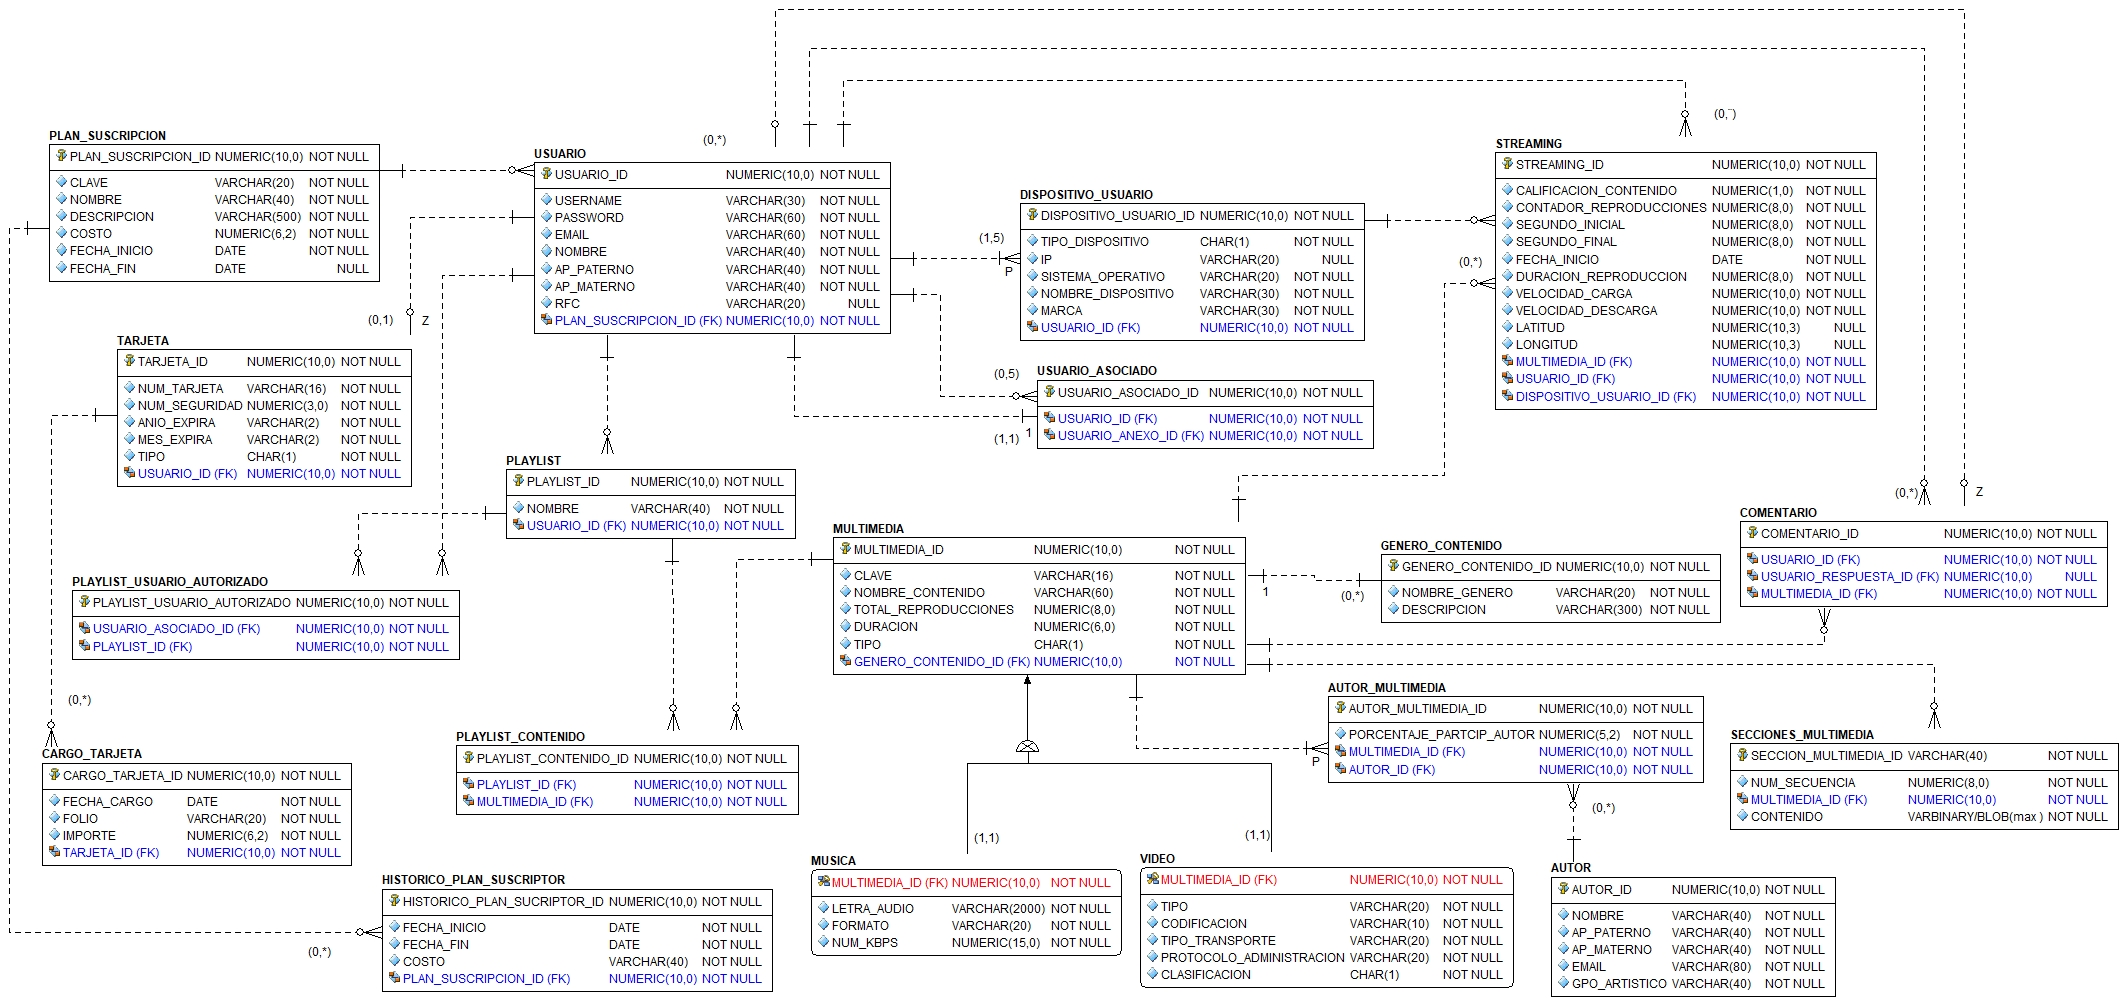
\includegraphics[width=0.95\textheight,angle=90]{media-stream-modelo-global}
\end{center}


\section*{Modelo relacional por módulo}

\textbf{Módulo 01:} Contenido multimedia (\textit{multimedia})

\begin{center}
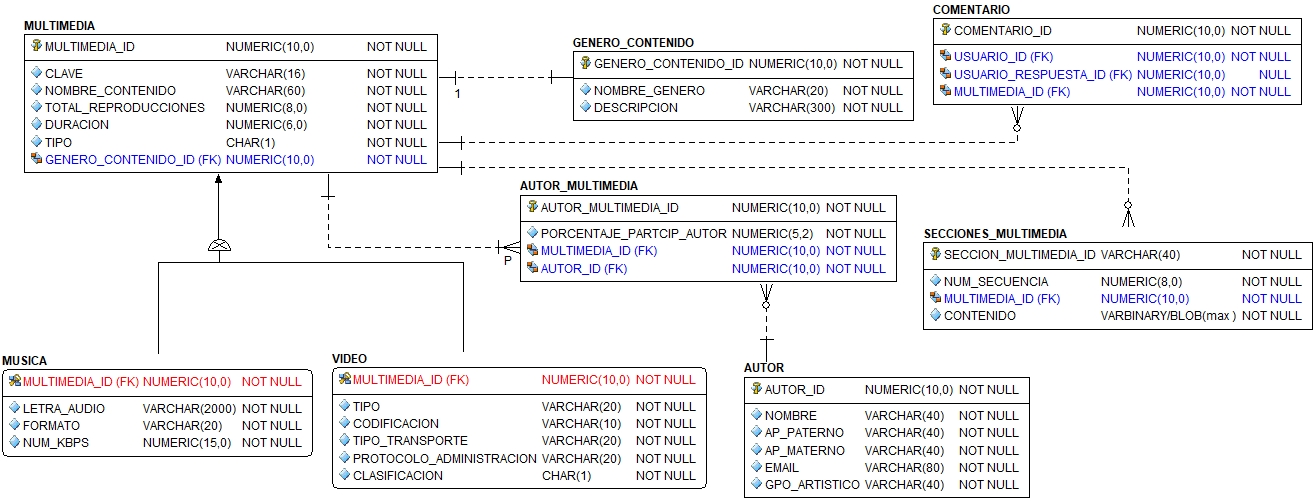
\includegraphics[width=0.95\textwidth]{media-stream-modulo-01}
\end{center}

\textbf{Módulo 02:} Streaming - Usuarios (\textit{users})

\begin{center}
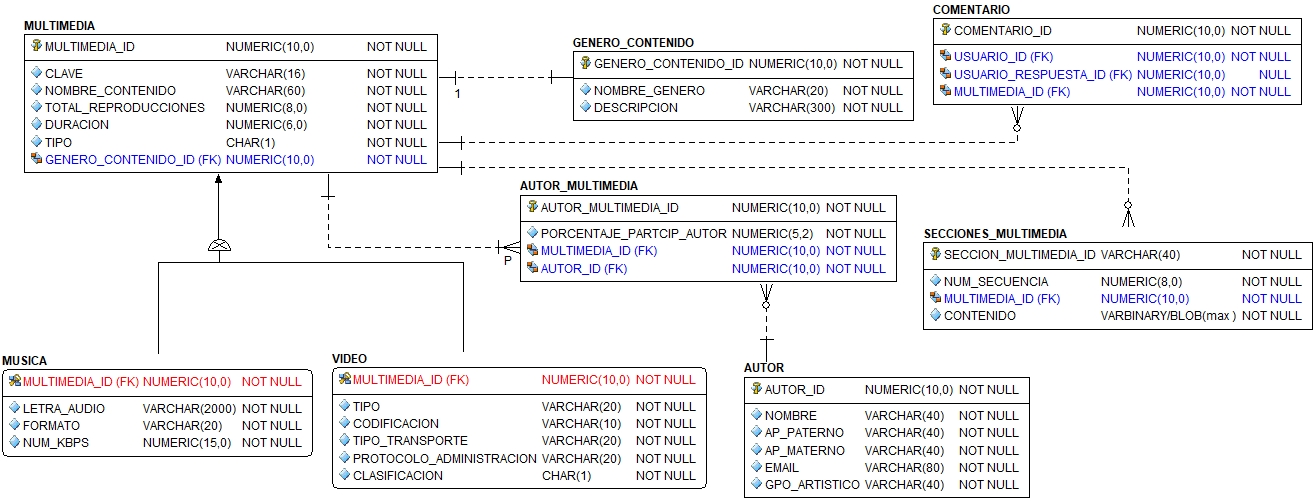
\includegraphics[width=0.95\textwidth]{media-stream-modulo-01}
\end{center}

\section{Diseño físico de la BD}

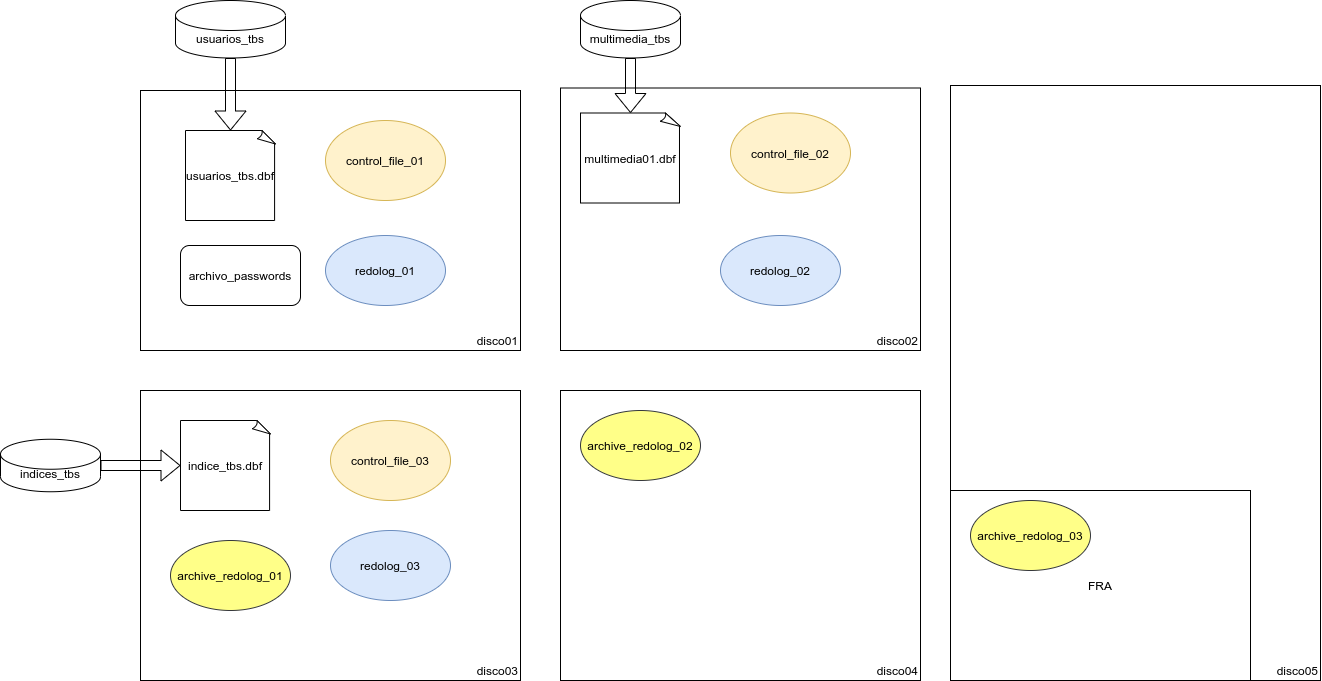
\includegraphics[width=0.9\textwidth]{arquitectura-bd-mediastream.png}

\subsection{Definición de tablespaces comunes a los módulos}

{
  \setlength\tabcolsep{3.5mm}
  \def\arraystretch{2}          % Do not define globally (for that reason we
                                % enclose table inside brackets)
  \begin{longtable}{
    |p{0.27\linewidth}
    |p{0.64\linewidth}|}
  \hline
  %%%%% Start: Table header 
  \textbf{Nombre del tablespace} & 
  \textbf{Configuración}
  \\ \hline
  %%%%% End: Table header 
  %
  % row 1
  undotbs1 & 
  \parbox[t][][t]{\linewidth}{
    \texttt{%
    undo tablespace undotbs1\\
    datafile `/u01/app/oracle/oradata/frpaproy/undotbs01.dbf'\\
    size 200m reuse autoextend on next 5120k maxsize unlimited;\\
    }
  }
  \\ \hline
  % row 2
  temptbs1 & 
  \parbox[t][][t]{\linewidth}{
    \texttt{%
    default temporary tablespace tempts1\\
    tempfile `/u01/app/oracle/oradata/frpaproy/temp01.dbf'\\
    size 20m reuse autoextend on next 640k maxsize unlimited\\
    }
  }
  \\ \hline
  \end{longtable}
}

\subsection{Definición de tablespaces por módulo}

{
  \setlength\tabcolsep{3.5mm}
  \def\arraystretch{2}          % Do not define globally (for that reason we
                                % enclose table inside brackets)
  \begin{longtable}{
    |C{0.23\linewidth}
    |p{0.4\linewidth}
    |C{0.24\linewidth}|}
  \hline
  %%%%% Start: Table header 
  \textbf{Nombre del tablespace} & 
  \textbf{Objetivo / Beneficio} & 
  \textbf{Tipo}
  \\ \hline
  %%%%% End: Table header 
  %
  % row 1
  users\_tbs & 
  Almacenar todos los datos referidos a los usuarios (tarjeta, plan de
  suscripción, playlist, pagos y dispositivos) así como también la información
  del consumo de contenido por streaming & 
  Permanente y small file% 
  \\ \hline
  % row 2 
  multimedia\_tbs &
  Almacenar los datos referidos al contenido multimedia de mediaStream. Este
  módulo permite almacenar datos BLOB y CLOB de manera independiente a los
  datos del usuario. &
  Permanente y bigfile
  \\ \hline
  \end{longtable}
}

\subsection{Configuración de tablespaces por módulo}

{
  \setlength\tabcolsep{3.5mm}
  \def\arraystretch{2}          % Do not define globally (for that reason we
                                % enclose table inside brackets)
  \begin{longtable}{
    |p{0.27\linewidth}
    |p{0.65\linewidth}|}
  \hline
  %%%%% Start: Table header 
  \textbf{Nombre del tablespace} & 
  \textbf{Configuración}
  \\ \hline
  %%%%% End: Table header 
  %
  % row 1
  users\_tbs & 
  % 
  \\ \hline
  % row 2
  multimedia\_tbs & 
  % 
  \\ \hline
  \end{longtable}
}

\subsection{Asignación de tablespace por tablas de cada módulo}

{
  \setlength\tabcolsep{3.5mm}
  \def\arraystretch{2}          % Do not define globally (for that reason we
                                % enclose table inside brackets)
  \begin{longtable}{
    |p{0.42\linewidth}
    |C{0.5\linewidth}|}
  \hline
  %%%%% Start: Table header 
  \textbf{Nombre de la tabla} & 
  \textbf{Nombre del tablespace}
  \\ \hline
  %%%%% End: Table header 
  %
  % row 9
  CARGO\_TARJETA & 
  users\_tbs% 
  \\ \hline
  % row 10
  DISPOSITIVO\_TARJETA & 
  users\_tbs% 
  \\ \hline
  % row 11
  HISTORICO\_PLAN\_SUSCRIPTOR & 
  users\_tbs% 
  \\ \hline
  % row 12
  PLAN\_SUSCRIPTOR & 
  users\_tbs% 
  \\ \hline
  % row 13
  PLAYLIST & 
  users\_tbs% 
  \\ \hline
  % row 14
  PLAYLIST\_CONTENIDO & 
  users\_tbs% 
  \\ \hline
  % row 15
  PLAYLIST\_USUARIO\_AUTORIZADO & 
  users\_tbs% 
  \\ \hline
  % row 16
  STREAMING & 
  users\_tbs% 
  \\ \hline
  % row 17
  TARJETA & 
  users\_tbs% 
  \\ \hline
  % row 18
  USUARIO & 
  users\_tbs% 
  \\ \hline
  % row 19
  USUARIO\_ASOCIADO & 
  users\_tbs% 
  \\ \hline
  % row 1
  AUTOR & 
  multimedia\_tbs 
  \\ \hline
  % row 2
  AUTOR\_MULTIMEDIA & 
  multimedia\_tbs 
  \\ \hline
  % row 3
  COMENTARIO & 
  multimedia\_tbs 
  \\ \hline
  % row 4
  GENERO\_CONTENIDO & 
  multimedia\_tbs 
  \\ \hline
  % row 5
  MULTIMEDIA & 
  multimedia\_tbs 
  \\ \hline
  % row 6
  SECCIONES\_MULTIMEDIA & 
  multimedia\_tbs 
  \\ \hline
  % row 7
  MUSICA & 
  multimedia\_tbs 
  \\ \hline
  % row 8
  VIDEO & 
  multimedia\_tbs 
  \\ \hline

  \end{longtable}
}

\newpage

\subsection{Asignación de tablespace para índices de cada módulo}

{
  \setlength\tabcolsep{3.5mm}
  \def\arraystretch{2}          % Do not define globally (for that reason we
                                % enclose table inside brackets)
  \begin{longtable}{
    |C{0.2\linewidth}
    |C{0.12\linewidth}
    |C{0.16\linewidth}
    |C{0.16\linewidth}
    |C{0.16\linewidth}|}
  \hline
  %%%%% Start: Table header 
  \textbf{Nombre del índice} & 
  \textbf{Tipo de índice} & 
  \textbf{Nombre de la tabla} & 
  \textbf{Nombre de la columna} & 
  \textbf{Nombre del tablespace}
  \\ \hline
  %%%%% End: Table header 
  %
  % row n
  AUTOR\_EMAIL\_UK&
  Único &
  AUTOR &
  EMAIL&
  indexes\_tbs
  \\ \hline
  % row n
  AUTOR\_MULTIMEDIA \_AUTOR\_ID\_FK &
  Referencia &
  AUTOR\_MULTIMEDIA &
  AUTOR\_ID& 
  indexes\_tbs
  \\ \hline
  % row n
  AUTOR\_MULTIMEDIA \_MULTIMEDIA\_ID\_FK &
  Referencia &
  AUTOR\_MULTIMEDIA &
  MULTIMEDIA\_ID& 
  indexes\_tbs
  \\ \hline
  % row n
  CARGO\_TARJETA \_TARJETA\_ID\_FK &
  Referencia &
  CARGO\_TARJETA &
  TARJETA\_ID& 
  indexes\_tbs
  \\ \hline
  % row n
  CARGO\_TARJETA \_FOLIO\_UK &
  Único &
  CARGO\_TARJETA &
  FOLIO&
  indexes\_tbs
  \\ \hline
  % row n
  COMENTARIO \_MULTIMEDIA\_ID\_FK &
  Referencia &
  COMENTARIO &
  MULTIMEDIA\_ID& 
  indexes\_tbs
  \\ \hline
  % row n
  COMENTARIO \_USUARIO\_ID\_FK &
  Referencia &
  COMENTARIO &
  USUARIO\_ID& 
  indexes\_tbs
  \\ \hline
  % row n
  COMENTARIO\_USUARIO \_RESPUESTA\_ID\_FK &
  Referencia &
  COMENTARIO &
  USUARIO\_RESPUESTA\_ID& 
  indexes\_tbs
  \\ \hline
  % row n
  DISPOSITIVO\_USUARIO \_USUARIO\_ID\_FK &
  Referencia &
  DISPOSITIVO\_USUARIO &
  USUARIO\_ID& 
  indexes\_tbs
  \\ \hline
  % row n
  HIST\_PLAN \_SUSCRIPTOR\_PLAN \_SUSCRIPTOR\_ID\_FK &
  Referencia &
  HISTORICO\_PLAN \_SUSCRIPTOR &
  PLAN \_SUSCRIPTOR\_ID& 
  indexes\_tbs
  \\ \hline
  % row n
  MULTIMEDIA\_GENERO \_CONTENIDO\_ID\_FK &
  Referencia &
  MULTIMEDIA\_GENERO &
  CONTENIDO\_ID& 
  indexes\_tbs
  \\ \hline
  % row n
  MULTIMEDIA\_GENERO \_CONTENIDO\_ID\_FK &
  Referencia &
  MULTIMEDIA\_GENERO &
  CONTENIDO\_ID& 
  indexes\_tbs
  \\ \hline
  % row n
  PLAN\_SUSCRIPTOR \_CLAVE\_UK &
  Único &
  PLAN\_SUSCRIPTOR &
  CLAVE&
  indexes\_tbs
  \\ \hline
  % row n
  PLAYLIST\_CONTENIDO \_MULTIMEDIA\_ID\_FK &
  Referencia &
  PLAYLIST\_CONTENIDO &
  MULTIMEDIA\_ID& 
  indexes\_tbs
  \\ \hline
  % row n
  PLAYLIST\_CONTENIDO \_PLAYLIST\_ID\_FK &
  Referencia &
  PLAYLIST\_CONTENIDO &
  PLAYLIST\_ID& 
  indexes\_tbs
  \\ \hline
  % row n
  PLAYLIST\_CONTENIDO \_PLAYLIST \_MULTIMEDIA\_IX &
  Compuesto &
  PLAYLIST\_CONTENIDO &
  PLAYLIST\_ID, MULTIMEDIA\_ID&
  indexes\_tbs
  \\ \hline
  % row n
  PLAYLIST\_USU\_AUT \_PLAYLIST\_ID\_FK &
  Referencia &
  PLAYLIST\_USUARIO \_AUTORIZADO &
  PLAYLIST\_ID& 
  indexes\_tbs
  \\ \hline
  % row n
  PLAYLIST\_USU\_AUT \_USUARIO \_ASOCIADO\_ID\_FK &
  Referencia &
  PLAYLIST\_USUARIO \_AUTORIZADO &
  USUARIO \_ASOCIADO\_ID& 
  indexes\_tbs
  \\ \hline
  % row n
  PLAYLIST\_USUARIO \_ID\_FK &
  Referencia &
  PLAYLIST &
  USUARIO\_ID& 
  indexes\_tbs
  \\ \hline
  % row n
  SECCIONES\_MULTIMEDIA \_MULTIMEDIA\_ID &
  Referencia &
  SECCIONES\_MULTIMEDIA &
  MULTIMEDIA\_ID& 
  indexes\_tbs
  \\ \hline
  % row n
  STREAMING\_DISPOSITIVO \_USUARIO\_ID\_FK &
  Referencia &
  STREAMING &
  USUARIO\_ID& 
  indexes\_tbs
  \\ \hline
  % row n
  STREAMING\_MULTIMEDIA \_MULTIMEDIA\_ID\_FK &
  Referencia &
  STREAMING &
  MULTIMEDIA\_ID& 
  indexes\_tbs
  \\ \hline
  % row n
  STREAMING\_MUTIMEDIA \_USUARIO\_IX &
  Compuesto &
  STREAMING &
  MULTIMEDIA\_ID, USUARIO\_ID& 
  indexes\_tbs
  \\ \hline
  % row n
  STREAMING\_USUARIO\_ID\_FK &
  Referencia &
  STREAMING &
  USUARIO\_ID& 
  indexes\_tbs
  \\ \hline
  % row n
  TARJETA\_USUARIO\_ID\_FK &
  Referencia &
  TARJETA &
  USUARIO\_ID& 
  indexes\_tbs
  \\ \hline
  % row n
  TARJETA\_NUM\_TARJETA\_UK &
  Único &
  TARJETA &
  NUM\_TARJETA& 
  indexes\_tbs
  \\ \hline
  % row n
  USUARIO\_ASOCIADO \_USUARIO\_ANEXO\_ID\_FK &
  Referencia &
  USUARIO\_ASOCIADO &
  USUARIO\_ANEXO\_ID& 
  indexes\_tbs
  \\ \hline
  % row n
  USUARIO\_ASOCIADO \_USUARIO\_ID\_FK &
  Referencia &
  USUARIO\_ASOCIADO &
  USUARIO\_ID& 
  indexes\_tbs
  \\ \hline
  % row n
  USUARIO\_PLAN \_SUSCRIPTOR\_ID\_FK &
  Referencia &
  USUARIO &
  SUSCRIPTOR\_ID& 
  indexes\_tbs
  \\ \hline
  % row n
  USUARIO\_USERNAME\_UK &
  Único &
  USUARIO &
  USERNAME& 
  indexes\_tbs
  \\ \hline
  % row n
  USUARIO\_EMAIL\_UK &
  Único &
  USUARIO &
  EMAIL& 
  indexes\_tbs
  \\ \hline
  % row n
  USUARIO\_RFC\_UK &
  Único &
  USUARIO &
  RFC& 
  indexes\_tbs
  \\ \hline
 
  \end{longtable}
}

\subsection{Asignación de tablespaces para columnas CLOB/BLOB de cada módulo}

{
  \setlength\tabcolsep{3.5mm}
  \def\arraystretch{2}          % Do not define globally (for that reason we
                                % enclose table inside brackets)
  \begin{longtable}{
    |C{0.16\linewidth}
    |C{0.16\linewidth}
    |C{0.16\linewidth}
    |C{0.16\linewidth}
    |C{0.15\linewidth}|}
  \hline
  %%%%% Start: Table header 
  \textbf{Nombre de la columna CLOB/BLOB} & 
  \textbf{Nombre de índice asociado a la columna CLOB/BLOB} & 
  \textbf{Nombre de la tabla} & 
  \textbf{Nombre del tablespace para la columna CLOB/BLOB} & 
  \textbf{Nombre del tablespace para el índice de la columna CLOB/BLOB}
  \\ \hline
  %%%%% End: Table header 
  %
  % row 1
  contenido &
  secciones\_multimedia \_contenido\_ix\_blob&
  SECCIONES\_MULTIMEDIA&
  multimedia\_tbs&
  contenido\_blob\_tbs% 
  \\ \hline
  \end{longtable}
}

%\section{Simulación de carga diaria}

%{
  %\setlength\tabcolsep{3.5mm}
  %\def\arraystretch{2}          % Do not define globally (for that reason we
                                %% enclose table inside brackets)
  %\begin{longtable}{
    %|C{0.16\linewidth}
    %|C{0.16\linewidth}
    %|C{0.16\linewidth}
    %|C{0.16\linewidth}
    %|C{0.15\linewidth}|}
  %\hline
  %%%%%% Start: Table header 
  %\textbf{Fecha y hora} & 
    %\textbf{Datos REDO producidos (MB)} & 
  %\textbf{Fecha de respaldo} & 
  %\textbf{Tipo de backup} & 
  %\textbf{Espacio requerido por el backup}
  %\\ \hline
  %%%%%% End: Table header 
  %%
  %% row 1
  %Hola &
  %Hola &
  %Hola &
  %Hola &
  %Hola% 
  %\\ \hline
  %\end{longtable}
%}




\end{document}
